\section{Proposed Approach}
\label{sec:approach}

\subsection{Multilingual CTC Model}
\begin{figure}[t]
    \centering
    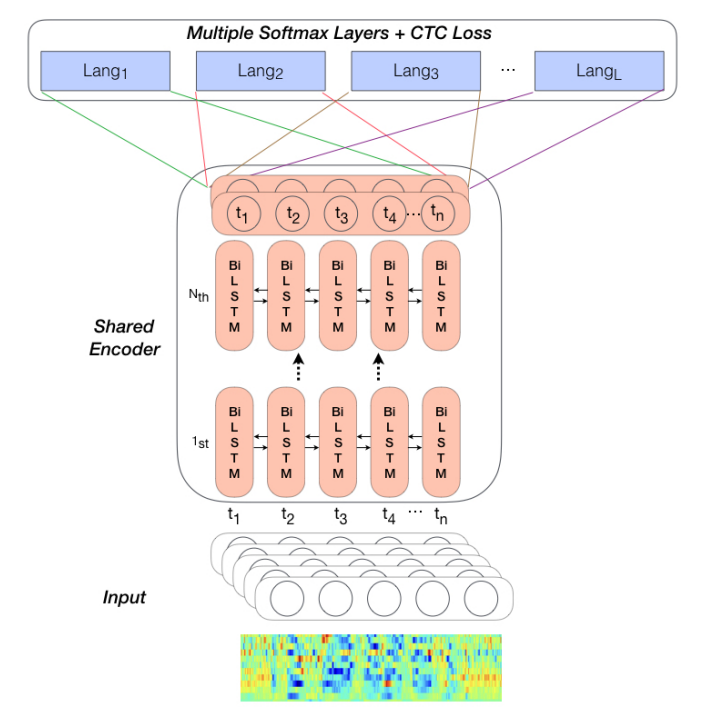
\includegraphics[width=\linewidth]{figs/model_arch.png}
    \caption{Multilingual CTC Model Architecture \textcolor{red}{WILL BE REPLACED}}
    \label{fig:model-arch}
    %\vspace{-10pt}
\end{figure}

We used the model architecture as illustrated in Fig.~\ref{fig:model-arch}, the shared encoder is parameterized by $\theta$, and the set of language-specific heads are parameterized by $\theta_h$ ($\theta_{h,l}$ means the head for $l$-th language). Let the dataset be $D$, composed of paired data $(X,C)$. Let $X = x_1, x_2, \cdots, x_T$ with length $T$ as input feature, $C = c_1, c_2, \cdots, c_L$ with length $L$ as target label. $X$ is encoded into sequence of hidden states $H = h_1, h_2, \cdots, h_{L^\prime}$ with length $L^\prime$ through the shared encoder, then fed into the language-specific head of the corresponding language with softmax activation to output the prediction sequence $\hat{C} = \hat{c_1}, \hat{c_2}, \cdots, \hat{c_{L^\prime}}$.
%\vspace{-2pt}

\textbf{CTC Loss}. CTC computes the posterior probability as below,

\begin{equation}
  P(C|X) = \sum_{\pi \in \mathcal{Z}(C)} P(\pi|X)
\end{equation}
where $\pi$ is the repeated character sequence  of $C$ with additional blank label, and $\mathcal{Z}(C)$ is the set of all possible sequences $\pi$ given sequence $C$. For each $\pi$, we can approximate the posterior probability as below,

\begin{equation}
  P(\pi|X) \approx \prod_{i=1}^{L^\prime} P(\hat{c_i}|X)
\end{equation}

The loss function of the model on $D$ is then defined as:

\begin{equation}
  \label{eq:ctc-loss}
  \mathcal{L}_D(\theta, \theta_h) = - \log P(C|X)
\end{equation}

\subsection{Meta Learning for Low-Resource ASR}

The idea of MAML is to learn initialization parameters from a set of tasks. 
In the context of ASR, we can view different languages as different tasks.
Given a set of source tasks $\mathcal{D}=\lbrace D_1, D_2, \cdots, D_K \rbrace$, MAML learns from $\mathcal{D}$ to obtain good initialization parameters $\theta^{\star}$ for the shared encoder.
$\theta^{\star}$ yields fast task-specific learning (fine-tuning) on target task $D_t$ and obtains $\theta^{\star}_t$ and $\theta^{\star}_{h,t}$ (the parameters obtained after fine-tuning on $D_t$). 
MAML can be formulated as below, 
\begin{equation*}
  \theta^{\star}_t, \theta^{\star}_{h,t} = \texttt{Learn}(D_t;\theta^{\star}) = \texttt{Learn}(D_t;\texttt{MetaLearn}(\mathcal{D})).
\end{equation*}
The two functions,  \texttt{Learn} and \texttt{MetaLearn}, will be described in the following two subsections.
%where $\theta^{\star}_t$ is the parameter obtained after fine-tuning on $T_t$.


\subsubsection{Learn: Language-specific learning}
Given any initial parameters $\theta^0$ of the shared encoder (either random initialized or obtained from pretrained model) and the data $D_t$. The language-specific learning process is to minimize the CTC loss function defined in Eq.~\ref{eq:ctc-loss}.

\begin{equation}
  \label{eq:fine-tune}
  \resizebox{0.91\hsize}{!}{$
\begin{aligned}
  \theta^\prime, \theta^\prime_{h,t} = \texttt{Learn}(D_t;\theta^0) & = \arg \, \min_{\theta, \theta_{h,t}} \mathcal{L}_{D_t}(\theta, \theta_{h,t}) \\
                                                                    & = \arg \, \min_{\theta, \theta_{h,t}} \sum_{(X,C) \in D_t} -\log P(C|X)
\end{aligned}
$}
\end{equation}
\begin{table*}[ht!]
\centering
\caption{Character (\% CER)  error rate w.r.t the pretraining languages set for all 4 target languages' FLP}
\label{tab:block-results}
\begin{tabular}{@{}ccccccccc@{}}
%\begin{tabular}{l|cc|cc|cc|cc}
\toprule
Model                                    & \multicolumn{2}{c}{Vietnamese}                         & \multicolumn{2}{c}{Swahili}                        & \multicolumn{2}{c}{Tamil}                        & \multicolumn{2}{c}{Kurmanji} \\

                                         & multi           & meta                                & multi           & meta                                & multi           & meta                                & multi           & meta           \\ \midrule
\multicolumn{1}{c|}{- (no-pretrain)}         & 100.0          & \multicolumn{1}{c|}{100.0}          & 100.0          & \multicolumn{1}{c|}{100.0}          & 100.0          & \multicolumn{1}{c|}{100.0}          & 100.0          & 100.0          \\

\multicolumn{1}{c|}{Bn Tl Zu}   & 53.2          & \multicolumn{1}{c|}{36.5}          & 52.8          & \multicolumn{1}{c|}{34.4}          & 47.8          & \multicolumn{1}{c|}{34.9}          & 55.9          & 41.1          \\
\multicolumn{1}{c|}{ Tr Lt Gn} & 50.6          & \multicolumn{1}{c|}{35.1}          & 49.0          & \multicolumn{1}{c|}{32.2}          & 46.6          & \multicolumn{1}{c|}{33.2}          & 53.4          & 39.6          \\
\multicolumn{1}{c|}{Bn Tl Zu Tr Lt Gn}           & 52.3          & \multicolumn{1}{c|}{36.6}          & 51.3          & \multicolumn{1}{c|}{33.0}          & 45.8          & \multicolumn{1}{c|}{33.9}          & 54.5          & 40.2          \\ \bottomrule
%\multicolumn{1}{c|}{MLing + SWBD \& FT}       & \textbf{48.2} & \multicolumn{1}{c|}{\textbf{33.5}} & \textbf{48.7} & \multicolumn{1}{c|}{\textbf{31.9}} & \textbf{44.3} & \multicolumn{1}{c|}{\textbf{31.9}} & \textbf{51.5} & \textbf{37.8} \\ \bottomrule
\end{tabular}
\end{table*}



The learning process is optimized through gradient descent, the same as MultiASR.

\subsubsection{MetaLearn}
The initialization parameters found by MAML should not only adapt to one language well, but for as many languages as possible. In order to achieve this goal, we define the meta learning process and the corresponding meta-objective as follows.

In each meta learning episode, we sample batch of tasks from $\mathcal{D}$, then sample two subsets from each task $k$ as training and testing set, denoted as $D_{k}^{tr}$, $D_{k}^{te}$, respecitvely. First, we use $D_k^{tr}$ to simulate the language-specific learning process to obtain $\theta^\prime_k$ and $\theta^\prime_{h,k}$.


\begin{equation}
    \theta_k^\prime, \theta_{h,k}^\prime = \texttt{Learn}(D^{tr}_k; \theta)
                                         %&= \arg \, \min_{\theta, \theta_{h,k}} \mathcal{L}_{D^{te}_k}(\theta, \theta_{h,k})
\end{equation}

Then evaluate the effectiveness of the obtained parameters on $D_k^{te}$. The goal of MAML is to find $\theta$, the initialization weights of the shared encoder for fast adaptation, so the meta-objective is defined as

\begin{equation}
  \label{eq:meta-obj}
  \mathcal{L}^{meta}_{\mathcal{D}}(\theta) =  \mathbb{E}_{k \sim \mathcal{D}} \; \mathbb{E}_{D_k^{tr}, D_k^{te}} \Big [ \mathcal{L}_{D^{te}_k}(\theta^\prime_k, \theta^\prime_{h,k}) \Big ]
\end{equation}

Therefore, the meta learning process is to minimize the loss function defined in Eq.~\ref{eq:meta-obj}.

\begin{equation}
  \theta^\star = \texttt{MetaLearn}(\mathcal{D}) = \arg \min_{\theta} \mathcal{L}^{meta}_{\mathcal{D}} (\theta)
\end{equation}

We use \textit{meta gradient} obtained from Eq.~\ref{eq:meta-obj} to update the model through gradient descent (\textit{outer loop}).

\begin{equation}
  \label{eq:meta-grad}
  \theta \leftarrow \theta - \eta^\prime \sum_k \nabla_\theta \mathcal{L}_{D^{te}_k}(\theta^\prime_k, \theta^\prime_{h,k})
\end{equation}
$\eta^\prime$ is the meta learning rate. And noted that only the shared encoder is updated via Eq.~\ref{eq:meta-grad}.

MultiASR optimizes the model according to Eq.~\ref{eq:fine-tune} on all source languages directly, without considering how learning happens on the unseen language. Although the parameters found by MultiASR is good for all source languages, it may not adapt well on the target language. Unlike MultiASR, MetaASR explicitly integrates the learning process into its framework via simulating language-specific learning first, then meta-update the model. Therefore,the parameters obtained are more suitable to adapt to the unseen language. We illustrated the concept in Fig.~\ref{fig:meta-idea}, and showed in the experimental results in Section \ref{sec:results}.


